\subsection{Derivación ferroviaria}

Cuando es necesario interconectar dos puntos separados por una distancia de decenas o cientos de kilómetros donde hay poco tráfico ferroviario, resulta económicamente poco conveniente construir vías en ambos sentidos. No obstante, construir una sola vía bidireccional presenta inconvenientes logísticos notorios: una formación que circule entre los puntos A y B excluye a cualquier formación que quiera circular de B a A sin colisionar. %No sería posible utilizar la infraestructura en el sentido opuesto mientras se encuentre ocupada.

La solución mas utilizada emplea islas de enclavamiento a modo de bypass cada cierta cantidad de kilómetros, como se ilustra en la Figura \ref{fig:bypass_1}. Estas islas permiten que las formaciones puedan cruzarse sin riesgo de colisión. La primer formación en llegar a la isla de enclavamientos accede al bypass por la vía superior y espera a que la formación en sentido contrario circule por la vía inferior. Una vez despejado el camino que resta por recorrer, la formación reingresa a la vía principal y retoma su marcha.

    \begin{figure}[H]
        \centering
        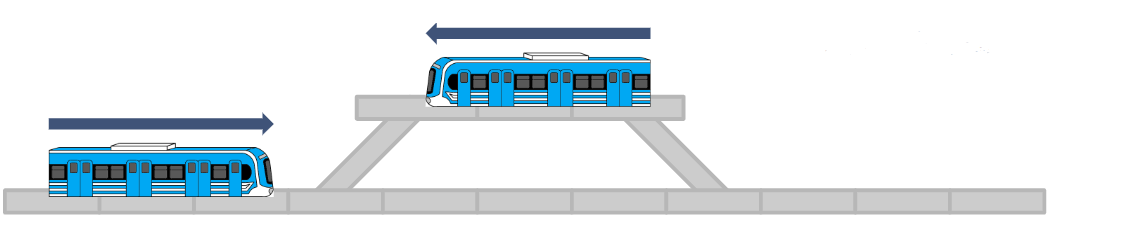
\includegraphics[width=1\textwidth]{Figuras/bypass}
        \centering\caption{Topología de derivación ferroviaria.}
        \label{fig:bypass_1}
    \end{figure}
    
Las topologías de derivación ferroviaria se utilizan principalmente para transportar materias primas entre locaciones rurales a grandes distancias de los puestos. Es deseable tanto una logística óptima, para transportar mas bienes y mas rápido, cómo un sistema seguro que garantice que los bienes lleguen a destino.